\documentclass[11pt]{book}
%% Packages élémentaires %%
\usepackage[utf8]{inputenc}
\usepackage{mathpazo,etoolbox, graphicx, wrapfig, pbox, fancybox, hyperref, appendix, geometry, amsmath, amssymb, tikz, pgfplots, calc, enumitem, colortbl
}
\newcommand{\cst}{\text{c}^{\text{\scriptsize ste}}}
\newcommand{\ddx}{\dfrac{\textrm d ^2 x}{\textrm d t^2}}
\renewcommand{\d}{\mathrm{d}}
\newcommand{\dx}{\mathrm{d}x}
\newcommand{\dy}{\mathrm{d}y}
\newcommand{\dz}{\mathrm{d}z}
\newcommand{\dt}{\mathrm{d}t}
\newcommand{\dxp}{\mathrm{d}x'}
\newcommand{\dyp}{\mathrm{d}y'}
\newcommand{\dzp}{\mathrm{d}z'}
\newcommand{\dtp}{\mathrm{d}t'}
\newcommand{\dvx}{\mathrm{d}\vec x}
\newcommand{\dvxp}{\mathrm{d}\vec x'}
\newcommand{\ch}{\mathrm{ch}}
\newcommand{\sh}{\mathrm{sh}}
\renewcommand{\th}{\mathrm{th}}
\newcommand{\tg}{\mathrm{tg}}
\newcommand{\C}{\textbf{C} }
\newcommand{\Cpp}{\textbf{C}++ }
\newcommand{\ud}[3]{{#1}^{#2} _{\; {#3} }}
\newcommand{\du}[3]{{#1}_{#2} ^{\; {#3} }}
\newcommand{\dd}[3]{{#1}_{#2} _{\; {#3} }}
\newcommand{\uu}[3]{{#1}^{#2} ^{\; {#3} }}
\setlength{\parindent}{0pt}

\graphicspath{{images/}}
\geometry{hmargin=2.4cm, vmargin = 2.1cm}
\setlist[itemize]{itemsep=10pt, label={--}}

%% Couleurs %%
\usepackage{xcolor}
\definecolor{bleu}{RGB}{14, 68, 175}
\definecolor{BGbleu}{RGB}{222, 233, 255 }
\definecolor{BGorange}{RGB}{255, 216, 154}
\definecolor{rouge}{RGB}{201, 0, 0}
\definecolor{vert}{RGB}{14, 137, 0}
\definecolor{BGgris}{RGB}{222,230,230}
\newcommand\rouge[1] {{\color{rouge}{#1}}}
\newcommand\bleu[1] {{\color{bleu}{#1}}}
\newcommand\green[1]{{\color{vert}{#1}}}


%% Cadres %%
\newcommand\bbm[1]{
\begin{center}
\fcolorbox{black}{BGbleu}{\parbox{\linewidth}{ 
#1
}}
\end{center}}
\newcommand\bo[1]{
\begin{center}
\fcolorbox{black}{BGorange}{\parbox{\textwidth}{ 
#1
}}
\end{center}}

\newcommand\bb[1]{
\begin{center}
\fcolorbox{black}{BGbleu}{\parbox{\textwidth}{ 
\begin{Large}
\begin{center}
#1
\end{center}
\end{Large}
}}
\end{center}}
\renewcommand\bo[1]{
\begin{center}
\fcolorbox{black}{BGorange}{\parbox{\textwidth}{ 
#1
}}
\end{center}}

\newcommand\boite[1]{
\begin{center}
\fbox{\parbox{\textwidth}{#1}}
\end{center}}



\newcommand\aparte[1]{
\begin{center}
\fcolorbox{white}{BGgris}{\parbox{\linewidth}{ \textit{A parte} \\
#1 }}
\end{center}}
\newcommand\bg[2]{
\begin{center}
\fcolorbox{white}{BGgris}{\parbox{\linewidth}{\begin{large} \textit{#1} \end{large} \\

#2 }}
\end{center}}

\newcommand\exemple[1]{
\begin{center}
\fcolorbox{white}{BGgris}{\parbox{\linewidth}{ \textit{Exemple} \\
#1 }}
\end{center}}

%% Commandes %%
\newcommand\imp[1]{\underline{\textbf{#1}}}
\newcommand\eq[1]{\begin{large}
\begin{align*}
#1
\end{align*}
\end{large}}
%% Commandes fantaisistes (cf. Internet) %%
\renewcommand{\parallel}{ \mathbin{\!/\mkern-5mu/\!} }
\newcommand{\q}[1]{{%
\font\larm = larm1000%
\larm%
\char 190}{ \textit{#1} }{%
\font\larm = larm1000%
\larm%
\char 191}}

%% Wrapping %%
\newcommand\wrap[4]{\begin{wrapfigure}[#1]{#2}{#3\textwidth}
#4
\end{wrapfigure}}
%% TikZ
\usepackage{pgfplots}
\usetikzlibrary{shapes}
\usetikzlibrary{calc}
\usetikzlibrary{positioning}
\usetikzlibrary{intersections}
\usetikzlibrary{angles}
\usetikzlibrary{quotes}
\newcommand{\drawaxes}[3]{
\coordinate (o) at #1 ;
\draw[->] ($(o) + (-0.1*#2, 0)$) --+ (#2, 0) ;
\draw[->] ($(o) + (0,-0.1*#3)$) --+ (0,#3) ;
}

\newcommand{\drawthickaxes}[5]{
\coordinate (o) at #1 ;
\draw[thick,->] ($(o) + (-0.1*#2, 0)$) --+ (#2, 0) node[anchor = north east]{#4};
\draw[thick,->] ($(o) + (0,-0.1*#3)$) --+ (0,#3) node[anchor = north east]{#5};
}

\newcommand*{\ShowIntersectionWithSinAbs}{
\fill 
    [name intersections={of=DroiteK and SinAbs, name=i, total=\t}] 
    [red, opacity=1, every node/.style={above left, black, opacity=1}] 
    \foreach \s in {1,...,\t}{
        \ifodd \s 
        {}
        \else
        (i-\s) circle (2pt) node [above] {\s} 
        \fi 
        };
}
\newcommand*{\ShowIntersectionWithCosAbs}{
\fill 
    [name intersections={of=DroiteK and CosAbs, name=i, total=\t}] 
    [blue, opacity=1, every node/.style={above left, black, opacity=1}] 
    \foreach \s in {1,...,\t}{
        \ifodd \s 
        (i-\s) circle (2pt) node [above] {\s} 
        \fi 
        };
}

%% Code %%
\usepackage{listings}
\definecolor{codegreen}{rgb}{0,0.6,0}
\definecolor{codegray}{rgb}{0.5,0.5,0.5}
\definecolor{codepurple}{rgb}{0.58,0,0.82}
\definecolor{backcolour}{RGB}{242,242,242}
\definecolor{codeorange}{RGB}{255,140,0}
% https://gist.github.com/nhtranngoc/88b72d9bfb656a3de227eea38ed80627
\definecolor{background}{RGB}{39, 40, 34}
\definecolor{string}{RGB}{230, 219, 116}
\definecolor{comment}{RGB}{117, 113, 94}
\definecolor{normal}{RGB}{248, 248, 242}
\definecolor{identifier}{RGB}{166, 226, 46}

\newcommand{\code}[1]{\texttt{{\color{codepurple}{#1}}}}
\newcommand{\codep}[1]{\texttt{{\color{codegreen}{#1}}}}

\lstdefinestyle{mystyle}{
    backgroundcolor=\color{backcolour},   
    commentstyle=\color{bleu},
    keywordstyle=\color{codeorange},
    numberstyle=\tiny\color{codegray},
    stringstyle=\color{codepurple},
    basicstyle=\ttfamily\footnotesize,
    breakatwhitespace=false,         
    breaklines=true,                 
    captionpos=b,                    
    keepspaces=true,                 
    numbers=left,                    
    numbersep=5pt,                  
    showspaces=false,                
    showstringspaces=false,
    showtabs=false,                  
    tabsize=2
}

\lstdefinestyle{py}{
	language=python,
    backgroundcolor=\color{backcolour},   
    commentstyle=\color{bleu},
    keywordstyle=\color{codeorange},
    numberstyle=\tiny\color{codegray},
    stringstyle=\color{codepurple},
    basicstyle=\ttfamily\footnotesize,
    breakatwhitespace=false,         
    breaklines=true,                 
    captionpos=b,                    
    keepspaces=true,                 
    numbers=left,                    
    numbersep=5pt,                  
    showspaces=false,                
    showstringspaces=false,
    showtabs=false,                  
    tabsize=2
}

\lstset{style=mystyle}
\lstset{language=C}

\lstdefinestyle{cppstyle}{
basicstyle=\footnotesize\sffamily\color{black},
commentstyle=\color{mygray},
frame=single,
numbers=left,
numbersep=5pt,
numberstyle=\tiny\color{mygray},
keywordstyle=\color{mygreen},
showspaces=false,
showstringspaces=false,
stringstyle=\color{myorange},
tabsize=2
}

\usepackage{framed}

\renewenvironment{leftbar}[1][\hsize]
{%
     \def\FrameCommand
     {%
         {\color{black}\vrule width 3pt}%
         \hspace{7pt}%must no space.
        % \fboxsep=\FrameSep\colorbox{yellow}%
     }%
     \MakeFramed{\hsize#1\advance\hsize-\width\FrameRestore}%
}
{\endMakeFramed}

\input{preambule-garde-2photos}
\newcommand\psirt{\psi(\vec{r},t)}
\newcommand\psikrt{\psi_{\vec{k}}(\vec{r},t)}
\newcommand\drawline[1]{%
     \begin{tikzpicture}                                                           
       \draw[#1] (0pt,0pt) -- (15pt,0pt);                                       
     \end{tikzpicture}%
} 

\documentname{Physique Quantique et Statistique}{B2-IRCI : PHYS-H2001 -- Pr. \textsc{Sparenberg}}{pqs-cover_1}{pqs-cover_2}
\author{Sami \textsc{Abdul Sater}}
\date{\hspace{-0.6cm}Année académique 2019-2020}
\begin{document}
\input{preambule-garde2}
\tableofcontents
\chapter{Introduction}\setcounter{page}{1}
\section{Fondements microscopiques de la physique}
Arrivés en BA2 Polytech, on a probablement compris que les lois de la physique sont les règles de ce monde, qu'absolument tout s'explique par elles. Les mêmes lois devraient alors pouvoir expliquer les phénomènes microscopiques et les phénomènes macroscopiques ! \\

\begin{itemize}
\item La \textit{physique quantique} est l'étude des lois \& propriétés du monde microscopique (particules élémentaires, noyaux atomiques, atomes, molécules).
\item La \textit{physique statistique} tente d'expliquer les lois du monde macroscopique par extrapolation de la physique quantique : moyennes de propriétés, etc. \\
\end{itemize}
Les différentes branches de la physique (mécanique, thermodynamique, électromagnétisme, optique, physique des matériaux) ne sont ainsi pas indépendantes : elles résultent du passage à l'échelle macroscopique des lois de la physique microscopique. Best phrase de 2020 so far. \\

L'interprétation qu'on a de la physique quantique repose sur 4 \textbf{principes fondamentaux}, qui peuvent être illustrés par un match de foot : \\
\bb{Principes fondamentaux de la physique
\begin{description}[leftmargin=!,labelwidth=\widthof{\bfseries Règles du jeu b}]
\item[Le terrain] L'espace-temps : $(x,y,z,t)$ (où ces coordonnées évoluent pour le décrire).
\item[Les joueurs] Les particules élémentaires, il y en a un petit nombre. On ne peut pas dissocier deux particules d'un même \textit{type} (deux électrons sont indiscernables par exemple).
\item[Le ballon] Les interactions que les particules s'échangent. Chaque interaction est caractérisée par des propriétés bien définies (portée, intensité, ...).
\item[Règles du jeu] Au cours des interactions, certaines  grandeurs ne sont pas modifiées : elles vérifient des \textit{lois de conservation} $\Rightarrow$ reliées à un principe de \textit{symétrie} dans l'univers.
\end{description}}
Avec ces principes on construit des hypothèses, des postulats. Un postulat est un fait qu'on ne peut pas démontrer, et qui permet surtout d'expliquer, de décrire \textbf{toutes} les observations expérimentales. Ils ne sont bien entendu pas définitifs.

\section{L'espace-temps et la relativité restreinte}
\q{Être là oslm} est une chose de signifiant dans l'espace-temps. En effet, \q{être là, à la position $\vec{r}$ à l'instant $t$} est une activité qui est décrite par un vecteur : un quadrivecteur en l'occurrence. Un quadrivecteur est un vecteur à 4 composantes équidimensionnelles qui vérifie certaines propriétés mathématiques plutôt joulies. Ce quadrivecteur traduit la présence à $(\vec{r},t)$ et est noté tout simplement :

\bb{Quadrivecteur évènement :\eq{(ct, x, y, z) \equiv (ct, \vec{r})}}

Pour une particule présente "là oslm" sa trajectoire dans l'espace temps est une droite.
\subsection{Référentiels inertiels}
La théorie de la relativité restreinte d'\textsc{Einstein} repose sur deux postulats. 
\begin{enumerate}
\item Pour deux référentiels en MRU l'un par rapport à l'autre, les lois de la physique sont les mêmes.
\item La vitesse de la lumière est la même dans tout référentiel.
\end{enumerate}  Elle a levé le doigt sur un aspect important : l'espace n'est guère différent du temps. Se mouvoir dans l'espace d'une certaine manière influence l'écoulement du temps. Ainsi, pour deux référentiels $\mathrm{R}$ et $\mathrm{R}'$, les temps $t$ et $t'$ sont \textit{a priori} des coordonnées différentes ! Graphiquement, on a un changement de repère de la manière qui suit , représenté sur la figure \textbf{\ref{fig:espace-temps}}.
\begin{figure}[h!]
\centering
\fbox{\parbox{\textwidth}{
\centering
    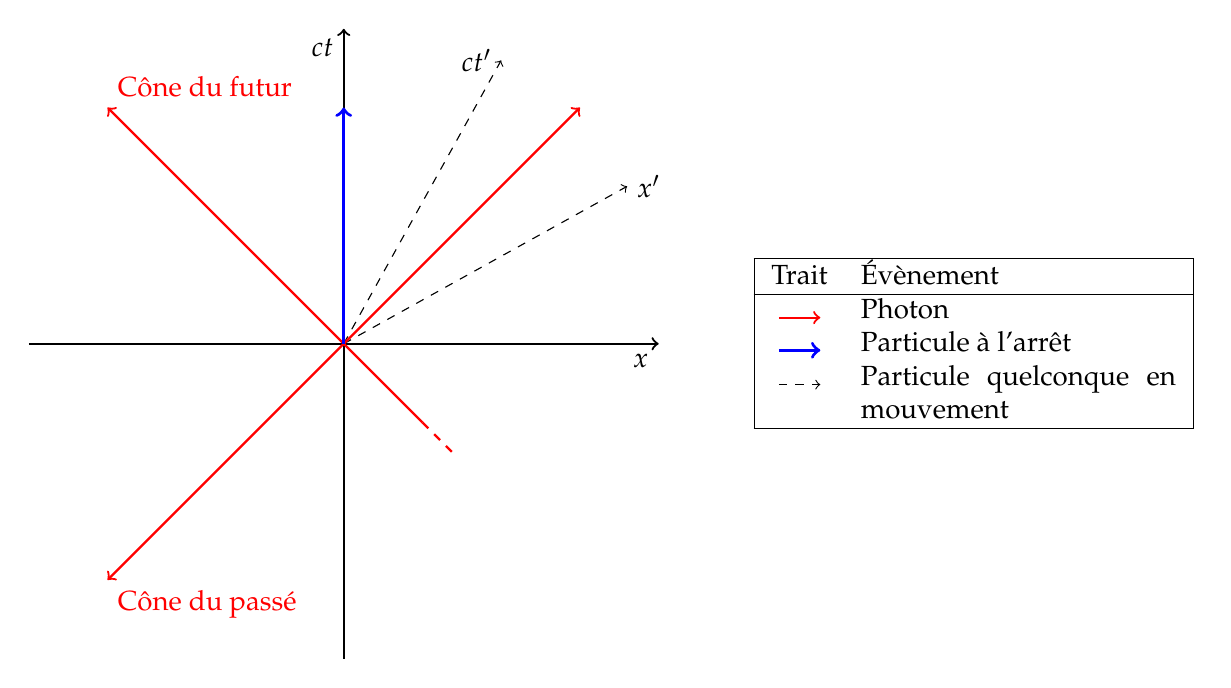
\begin{tikzpicture}
\draw[thick, ->] (-4,0) -- (4,0) node[anchor = north east]{$x$} ;
\draw[thick, ->] (0,-4) -- (0,4) node[anchor = north east]{$ct$} ;
\draw[->, dashed] (0,0) -- (3.6,2) node[anchor =  west]{$x'$} ;
\draw[->, dashed] (0,0) -- (2,3.6) node[anchor =  east]{$ct'$} ;
\draw[red,thick, <->](3,3) -- (-3, -3) node[anchor = north west]{Cône du passé} ;
\draw[red,thick, ->](1,-1) -- (-3, 3) node[anchor = south west]{Cône du futur} ;
\draw[red, thick, dashed] (1,-1) -- (1.4, -1.4) ;
\draw[blue,very  thick, ->] (0,0) -- (0,3) ;
\node (tab1) at (8,0) {%
  \begin{tabular}{|c p{4cm}|}
  \hline
  Trait & Évènement\\
  \hline 
\drawline{red,thick, ->} & Photon \\
\drawline{blue, very thick, ->} & Particule à l'arrêt \\
\drawline{dashed, ->} & Particule quelconque en mouvement \\
\hline
  \end{tabular}};
\end{tikzpicture}}}
    \caption{Représentation graphique de l'espace-temps tel que décrit dans la théorie de la relativité restreinte.}
    \label{fig:espace-temps}
\end{figure}
L'interprétation de cette figure est la suivante : plus la particule est rapide, plus ses axes se \q{resserrent} jusqu'à être confondus, à la vitesse maximale, celle du photon. \imp{Attention} : cette interprétation est trompeuse parce que dans l'espace-temps, les axes $O_{ct}$ et $O_{x_i}$ sont toujours orthogonaux !
\subsection{Quadrivecteurs}
Un quadrivecteur est un objet mathématique, un vecteur à 4 composantes qui ont la même dimension. On le note en toute généralité $\mathrm{A} \equiv (A_t, \vec{A})$. Lors d'un changement de référentiel, chaque composante change de référentiel.

\bb{Quadrivecteur : changement de référentiel\eq{\mathrm{A} := (A_t, \vec{A}) \longleftrightarrow (A_{t'}, \vec{A}') \equiv (A_{t'}, A_{x'}, A_{y'}, A_{z'}) =: \mathrm{A}'}}
\subsubsection{Produit scalaire entre quadrivecteurs}
\wrap{5}{r}{0.5}{
\begin{center}

\vspace{-1.5cm}
\begin{tabular}{|p{2cm}|p{2cm}|p{2.6cm}|}
\hline
$\mathrm{A}$ & Type & Exemple  \\
\hline
$\mathrm{A}^2 >0 $& Temps & $(ct,0,0)$ \\
$\mathrm{A}^2 <0 $& Espace & $(0, x, y, z)$ \\
$\mathrm{A}^2 =0 $& Lumière & $c^2 t^2 - r^2 = 0$ \\
\hline
\end{tabular}\end{center}}
Simple opération mathématique, de laquelle on tire des propriétés d'interprétation physique :

\eq{\mathrm{A} \circ \mathrm{B} = A_t B_t -  \sum_i A_{x_i} B_{x_i}}
Le produit scalaire de $\mathrm{A}$ avec lui même est par définition le carré du quadrivecteur, aussi appelé norme pseudo-euclidienne.

\eq{\mathrm{A}^2 := \mathrm{A} \circ \mathrm{A} = A_t ^2 - \sum_i  A_{x_i} ^2}

Le produit scalaire est \textbf{invariant} dans les référentiels. On peut donc calculer la norme pseudo-euclidienne dans n'importe quel référentiel.
\subsection{Quadrivecteur énergie-impulsion}
Il s'agit d'un quadrivecteur très important pour une particule de masse $m$ :

\bb{Quadrivecteur énergie-impulsion :\eq{\mathrm{P} :=(E/c, \vec{p})}}
L'impulsion $\vec{p}$ apparaît dans cette expression. Elle est liée à la vitesse par la formule

\eq{\vec{v} = \dfrac{c^2}{E} \vec{p}.}
Dans le référentiel où la particule est au repos, elle possède une énergie résiduelle non nulle comme conséquence de sa masse. Celle-ci est appelée \q{énergie de masse} et est notée $E_0$. Elle est donnée par $mc^2$. Dans un référentiel où la particule est en mouvement, son énergie est donnée par la somme de son énergie de masse et de son énergie cinétique $T$. On veut alors trouver l'énergie totale, qu'on note $E$. Seulement, on ne connaît pas l'énergie cinétique. Par contre, on peut exprimer $\mathrm{P}^2$ dans deux référentiels (\bleu{particule en mouvement}, \rouge{particule au repos}) différents et égaler les expressions pour avoir une expression de $E$ !
\eq{E = E_0 + T \quad \land \quad \mathrm{P}^2 = \bleu{E^2/c^2 - p^2} = \rouge{E_0 ^2/c^2 = m^2c^2} \quad \Rightarrow \quad \boxed{E = \sqrt{m^2c^4 + p^2c^2}}}
Grâce à la relation entre vitesse et impulsion, on peut réécrire l'énergie comme 
\eq{ E = \frac{mc^2}{\sqrt{1-v^2/c^2}}.}
Mais la forme encadrée est plus générale et meilleure à retenir. En effet, on peut y voir qu'une particule de masse nulle a une énergie $ E = cp$ ce qui n'est possible que pour une vitesse égale à $c$ (\textit{cf.} relation vitesse-impulsion).
\subsection{Cas particuliers}
\begin{itemize}
\item Domaine \textit{ultrarelativiste} ($p\gg mc$) : l'énergie de masse devient négligeable devant l'énergie cinétique. Toute particule peut devenir ultrarelativiste quand sa vitesse est proche de $c$.
\item Domaine \textit{non relativiste} ($p\ll mc$): on peut approximer la formule de l'énergie ci-dessous avec un développement du premier ordre en Taylor-Maclaurin.

\eq{E = \sqrt{m^2c^2 + p^2c^2} = mc^2 \left( 1 + \dfrac{p^2}{m^2c^2}\right)^{1/2} \approx mc^2 \left( 1 + \dfrac{p^2}{2m^2c^2}\right) = mc^2 + \rouge{\dfrac{p^2}{2m}}}
On voit alors apparaître le terme correspondant à l'\rouge{énergie cinétique en domaine non relativiste}.
\end{itemize}
\section{Le modèle standard des particules}
\wrap{13}{r}{0.5}{\centering\vspace{-0.5cm}\includegraphics[width=0.4\textwidth]{PQS-2}
\caption{Tableau des 12 particules élémentaires}}
Voici le tableau des particules élémentaires. Colonne I : matière stable, contrairement aux colonnes II et III, un peu plus \q{exotiques}. Les particules instables sont plus massives et demandent donc plus d'énergie pour les créer. Les particules des colonnes IV représentent les vecteurs des interactions, les \textit{bosons de jauge}. \\

À chaque particule on associe une \textit{antiparticule}, particule de même masse, même spin, mais charge opposée. \\
\begin{eqnarray*}
e^- &\leftrightarrow& e^+ \\
\nu_e &\leftrightarrow& \bar{\nu}_e \\
&\cdots&
\end{eqnarray*}
\subsection{Leptons}
Ce sont les particules insensibles à l'interaction nucléaire forte. Il s'agit des \textit{particules dépourvues de quarks}. Étant donné que l'interaction forte véhicule beaucoup d'énergie ($\Leftrightarrow$ masse), ces particules sont moins lourdes que celles comportant des quarks.
\subsection{Hadrons}
Les hadrons sont des particules composées de quarks. Ces-derniers ne se trouvent \textbf{jamais} seuls ! On les trouve soit par paquets de 2 (\textbf{mésons}) soit de 3 (\textbf{baryons}), comme le proton ($\mathrm{uud}$) ou le neutron ($\mathrm{udd}$). \\

Le proton et le neutron ayant des propriétés (même le spin !) très similaires (pas la charge du coup), on parlera de nucléon en toute généralité dans le cours. Le spin total vaut 1/2. \rouge{En outre, chose à retenir, le proton a une énergie de masse de 1 GeV.}

\section{Les quatre interactions fondamentales}
\begin{figure}[h!]
\centering
\includegraphics[width = 0.7\textwidth]{PQS-3}
\caption{Table tirée du cours de M. Sparenberg reprenant les interactions, leur caractère répulsif ou attractif, portée et intensité.}
\label{fig : interactions fond}
\end{figure}
\begin{description}[align=right, labelwidth = 3cm]
\item[Gravitationnelle] Faible et toujours attractive
\item[Électromagnétique] Cohésion des atomes \& molécules
\item[Nucléaire forte] Cohésions des noyaux atomiques 
\item[Nucléaire faible] Relie hadrons et leptons, explique la radioactivité $\beta$. Elle n'a aucun effet sur la matière mais explique la transformation d'un neutron en un proton (un quark d devient u en émettant un électron et un antineutrino électronique).
\end{description}
\section{Lois de conservation}
Lors d'une interaction, on peut observer que certaines grandeurs sont conservées. Cela nous amène à définir des lois de conservation \textit{pour une interaction}. Certaines sont déduites par \textit{symétrie} de la nature.
\subsection{Conservation de l'énergie}
L'énergie totale d'un système ne peut pas changer. À l'échelle microscopique, on a énergie de masse, cinétique, et potentielle. Tout ça peut s'échanger mais se \textbf{conserve}.
\subsection{Conservation de l'impulsion}
Étant donné qu'énergie et impulsion sont deux composantes d'un même objet, $\mathrm{P} \equiv (E/c, \vec{p})$, \textit{en relativité restreinte}, si l'énergie est conservée alors l'impulsion aussi.
\subsection{Conservation du moment cinétique}
Le moment cinétique est conservé lors d'une interaction. On verra par la suite que le moment cinétique en physique quantique est \textbf{quantifié}.
\subsection{Conservation de la charge et des nombres baryonique et leptonique}
Un baryon a un nombre baryonique $+1$, un antibaryon $-1$ et un lepton $0$. Le principe est le même pour le nombre leptonique. Au fait, la charge aussi est conservée lors d'une interaction.

\chapter{Les origines de la physique quantique}
Ce qui a poussé la communauté scientifique à penser que l'étude de la physique microscopique était loin d'être terminée, c'est surtout l'observation \textbf{expérimentale} de la dualité onde-particule de la lumière ainsi que de la matière.
\section{Dualité onde-particule pour la lumière}
\subsection{La lumière est une onde}
\subsubsection{Franges de Young}
\wrap{10}{r}{0.5}{\vspace{-0.5cm} \centering
\includegraphics[width = 0.44\textwidth]{PQS-4} }
L'expérience de Young a permis de \underline{démontrer} que la lumière est une onde, en construisant une figure d'interférence propre aux objets ondulatoires à partir d'un faisceau lumineux projeté sur un mur dans lequel sont percées deux fentes. La figure d'interférence est quelque chose de mathématique, la réalité physique correspondant est un ensemble de franges lumineuses. Là où la frange est lumineuse, c'est le siège d'une interférence constructive :

\eq{\text{Interférence constructive } \iff d\sin \theta = n \lambda \qquad n \in \mathbb{Z}}
On voit dans cette expression la condition mathématique d'interférence constructive, \textit{dans le cas où la lumière est une onde}. Une figure d'interférence est observée quand cette relation est vérifiée. On déduit alors que la lumière émise est un objet constitué de raies de longueur d'onde $\lambda$. 
\paragraph{Remarque.} L'angle $\theta$, qui représente l'angle entre l'horizontale et le lieu d'interférence constructive, dépend de la longueur d'onde de la lumière utilisée. En particulier, une lumière rouge ($\lambda \gg$) produira des maxima d'intensité très espacés, alors qu'une lumière verte ($\lambda \ll$) beaucoup moins espacés.
\subsubsection{Diffraction de Bragg}
Dans l'expérience de Young, on avait 2 fentes qui diffractaient. Dans l'expérience de Bragg, on fait passer un rayon X à travers un cristal, ce sont les couches du cristal vont créer la diffraction. On a donc une infinité de couches qui diffractent. L'intensité de la figure d'interférence obtenue est donc beaucoup plus forte !

\subsection{La lumière est faite de particules}
\subsubsection{La constante de Planck}
Max \textsc{Planck} étudiait les corps noirs (enceinte macroscopique à l'équilibre thermodynamique) et de ses études est ressorti un paramètre qui a les dimensions $\mathrm{E} \times \mathrm{T} \equiv \mathrm{Js}$ ou \textit{action}. Ce paramètre qu'on note $h$ décrit formidablement les propriétés des corps noirs. L'étude de Max Planck aboutissait à une conclusion que l'énergie d'un corps noir est quantifiée. De l'autre côté, Einstein décrit également \textbf{l'effet photoélectrique} \footnote{Effet expliquant l'émission d'électrons par un métal exposé à de la lumière dans certaines conditions.} avec cette constante. Ceci souligne l'importance de $h$ car le corps noir et le métal n'ont \textit{a priori} rien en commun. La constante de Planck est donc une des \textit{constantes de l'Univers}.

\eq{ h \approx 6.63 \ 10^{-34} \ \ \mathrm{Js}}
On définit similairement la \textit{constante de Planck réduite}, $\hbar$ :
\eq{\hbar := h/2\pi \approx 1.055 \ 10^{-34} \ \ \mathrm{Js}}
 Le lien formidable qui a été effectué par Einstein est l'extrapolation de la quantification de l'énergie, en stipulant simplement que \textbf{tout rayonnement est constitué de quanta d'énergie} lié à la fréquence du rayonnement. Le coefficient de proportionnalité est $h$
 \eq{E = h\nu = h \dfrac{\omega}{2\pi} \quad \Rightarrow \quad \boxed{E \equiv \hbar \omega}}
\subsubsection{Effet photoélectrique}
En bombardant une plaque métallique de lumière de longueur d'onde $\lambda$ (maintenant qu'on sait que la lumière est une onde), on remarque qu'au-delà d'une certaine fréquence $\nu_0$ ($\lambda$ et $\nu$ sont liées par $\lambda = c/\nu$), des électrons sont émis avec une énergie qui augmente linéairement avec la fréquence, avec une pente de $h$.

\eq{T = h\nu - W \qquad \text{où} \quad W = h\nu_0}
$W$ est le travail que fournit la lumière, l'énergie associée à un rayonnement de fréquence $\nu_0$.

\subsubsection{Les particules de lumière}
Einstein est amené à établir une relation entre la longueur d'onde de la lumière et une impulsion (à travers le nombre d'onde, ou plus précisément, le vecteur d'onde $\vec{k}$). Ce faisant, il donne aux quantas d'énergie toutes les propriétés d'une particule. Comme l'énergie et liée à la pulsation $\omega$ et l'impulsion est lié au vecteur d'onde $\vec{k}$, on peut lier le quadrivecteur $\mathrm{P}$ à un autre quadrivecteur, le \q{quadrivecteur d'onde} $\mathrm{K}$.
\begin{center}
$\left\{ \begin{array}{l}
E \equiv \hbar \omega \quad \text{\small (quantification de l'énergie}) \\
\vec{p} \equiv \hbar \vec{k}  \quad \text{\small (lien longueur d'onde-impulsion)}
\end{array} \right.
\qquad \Rightarrow \qquad 
\left\{ \begin{array}{l}
\mathrm{P} \equiv (E/c, \vec{p}) \\
\mathrm{K} \equiv (\omega/c, \vec{k})
\end{array} \right. \quad \Rightarrow \quad \boxed{\mathrm{P} = \hbar \mathrm{K}}$
\end{center}
Pour une particule de lumière, la relation de dispersion, c'est-à-dire le lien entre la pulsation et le nombre d'onde, est donnée par  $\omega = kc$. Ceci implique par la quantification de l'énergie $E = pc$, ce qui est la caractéristique d'une particule de masse nulle. La lumière est ainsi faite de particules de masse nulle. \\

L'introduction d'une particule de lumière, a.k.a le \textbf{photon} n'est pas super appréciée et nécessite donc d'être démontrée. C'est ce qu'a fait Arthur Compton expérimentalement. Il a démontré que lors d'une interaction (une collision) photon-électron, l'impulsion et l'énergie du photon étaient conservées, tout comme une particule classique. Le photon est donc bien une particule. Eeeet c'est aussi une onde (\textit{cf.} franges de Young). 
\begin{center}
\begin{large}
\textit{La lumière est donc une onde \underline{et} faite de particules.}
\end{large}
\end{center}

\subsection{Observation de la dualité onde-particule de la lumière}
On reprend l'expérience des fentes de Young et cette fois-ci en lumière atténuée, pour voir la figure d'interférence se construire progressivement. On alors les impacts un par un, \textbf{photon par photon} mais à long terme on voit se dessiner une figure d'interférence, cela veut dire que la lumière est une onde qui passe par les deux fentes à la fois.

\begin{itemize}
\item Nature corpusculaire : les impacts individuels.
\item Nature ondulatoire : la lumière passe par les deux fentes à la fois (figure d'interférence).
\item Dualité onde-particule : la lumière est à la fois partout et à un seul endroit. \end{itemize}
\section{Ordre et limites du spectre visible}
Dans l'ordre croissant :
\begin{enumerate}
\item Infrarouge, micro-ondes, ondes radio (qques km) : peu énergétiques et donc grande longueur d'onde
\item Lumière visible : au centre ($\lambda\approx 10^{-6}$m
\item UV : plus énergétique
\item X, Gamma : encore plus énergétique.
\end{enumerate}
\section{Dualité onde-particule de la matière}
\subsection{Longueurs d'onde (spectre) caractéristiques de matériaux | Expérience de Kirchoff}
Kirchoff en 1859 observe que le spectre de lumière émise et absorbée par un matériau est le même. En d'autres termes, il chauffe une enceinte de gaz et analyse le spectre de lumière émis. Il observe des maximas d'intensité pour certaines longueur d'ondes obtenues ($\equiv$ quantification de la longueur d'onde, du rayonnement, donc un spectre). Il observe de même pour la même enceinte lorsque traversée par de la lumière blanche (spectre dit \q{en absorption}) : des minimas d'intensité pour certaines longueurs d'onde. L'observation la plus choquante est que ces longueurs d'onde coïncident. Le spectre en absorption/en émission est une propriété du matériau. Explication mathématique par la formule de Rydberg : \textit{pour des atomes quelconques, l'inverse de la longueur d'onde est toujours une différence entre deux états}.

\eq{\dfrac{1}{\lambda_{n'n}} = R\left( \dfrac{1}{n'^2} - \dfrac{1}{n^2} \right)}
\subsection{Explication de de Broglie}
\begin{center}
\textit{Louis de Broglie a avancé l'hypothèse révolutionnaire qu'une onde est associée au mouvement de tous les types de particules, massiques ou non.}\end{center}
La suite de l'hypothèse de de Broglie est que toute onde qui accompagne une particule d'impulsion (dépendant donc de la vitesse) $p$ a une longueur d'onde $\lambda$ donnée par la formule suivante. En supposant de plus que l'onde se propage parallèlement à la vitesse (et donc à l'impulsion) de la particule, on obtient pour une onde de matière :
\eq{\lambda = h/p \quad \Rightarrow \boxed{\vec{p} = \hbar \vec{k}}}

Cette relation implique l'équivalence entre énergie et pulsation, $E = \hbar \omega$. La relation de dispersion est, en toute généralité, différente de $\omega = kc$.

\chapter{L'équation de Schrödinger}
\section{Approche déductive : à partir de l'onde électromagnétique}
L'électromagnétisme fut marqué par l'arrivée de la relativité restreinte. Celle-ci introduit notamment divers concepts et notations qui en simplifient beaucoup d'autres. On peut par exemple citer l'arrivée de la notion de \textit{quadrivecteur}, en particulier le \textit{quadrigradient} $\nabla$, sa notation en coordonnées covariantes\footnote{Le quadrigradient en coordonnées contravariantes $\partial^\mu$ fait apparaître un signe négatif devant les dérivées spatiales.} $\partial_\mu$ ou contravariantes $\partial^\mu$, et finalement le quadrivecteur potentiel $\mathrm{A}$ :
\eq{\boxed{\nabla \equiv \left(\frac{1}{c}\partial_t, \vec{\nabla}\right)} \ \ , \qquad \partial_\mu  \equiv \left(\frac{1}{c}\partial_t, \rouge{-}\partial_x, \rouge{-}\partial_y ,\rouge{-}\partial_z\right), \qquad \mathrm{A} \equiv \left(\frac{\mathrm{V}}{c}, A_x, A_y, A_z\right)}
qui permettent de concilier les 4 équations de Maxwell en une équation faisant intervenir le tenseur électromagnétique $\overline{\raisebox{0pt}[2.2ex]{$\overline{\raisebox{0pt}[1.8ex]{F}}$}}$ et le tenseur de Faraday $\overline{\raisebox{0pt}[2.2ex]{$\overline{\raisebox{0pt}[1.8ex]{J}}$}}$ :
\eq{\mathrm{F}^{\mu\nu} \equiv \rouge{\partial^\mu} \mathrm{A}^\nu -\partial^\nu \mathrm{A}^\mu, \qquad J^\nu \equiv (\rho c, J^x, J^y, J^z) \qquad \Longrightarrow \qquad \partial_\mu F^{\mu \nu} = \mu_0\mathrm{J}^\nu}
Mais l'important de ceci est ce qui est encadré : le quadrigradient. On remarque mis au carré dans le sens de la norme pseudo-euclidienne, on obtient un opérateur qui décrit une onde électromagnétique. On appelle cet opérateur \q{quadrilaplacien} ou \q{D'Alembertien}, et on le note $\Box$ :
\eq{\boxed{\Box := \nabla^2 = \dfrac{1}{c^2} \dfrac{\partial ^2}{\partial t^2} - \Delta} \qquad \boxed{\text{Onde électromagnétique :}\quad \Box \vec{B} = 0}}
On connaît diverses choses à propos de cette équation. Notamment, elle est :
\begin{itemize}
\item Linéaire
\item Vectorielle
\item Réelle
\end{itemize}
Et on connaît l'allure d'une solution de cette équation, il s'agit de la partie réelle d'une exponentielle complexe (négative) dont l'amplitude et la phase sont données par un phaseur. 
\begin{large}
\begin{equation}\label{eq:ondeEM}
\vec{B}_{\vec{k}}(\vec{r},t) = \text{Re}\left[\underline{\vec{B}_0}\ e^{i(\vec{k}\cdot\vec{r} - \omega t)} \right]
\end{equation}
\end{large}
On peut à partir de là faire deux choses :
\begin{enumerate}
\item Construire une solution générale, donc prendre les solutions (vectorielles) $\vec{B}_{\vec{k}}(\vec{r},t)$ et les sommer sur $\vec{k}$ en les pondérant d'une fonction $C(\vec{k})$ qui dépend de $\vec{k}$ en toute généralité :
\begin{large}
\begin{equation}\label{eq:ondeEMpaquet}
\vec{B}(\vec{r},t) = \int C(\vec{k})\ \vec{B}_{\vec{k}}(\vec{r},t) \ d\vec{k}
\end{equation}
\end{large}
\item Déduire une certaine règle de calcul, en remarquant que $\partial_t$ revient à multiplier par $-i\omega t$, et que $\vec{\nabla}$ revient à multiplier par $i\vec{k}$. En effet, écrire $\Box \vec{B} = 0$ revient alors à écrire :
\eq{\dfrac{1}{c^2} (-\omega^2) + k^2 = 0 \iff \boxed{\omega = kc}}
L'encadré est un lien entre la pulsation et le nombre d'onde, il s'agit de la relation de dispersion de l'onde. Cette relation porte ce nom parce que l'objet physique qu'est une onde \textit{plane} se disperse au cours du temps (et donc au travers de l'espace). On peut voir facilement dans l'équation \ref{eq:ondeEM} la vitesse de propagation d'une phase (la phase est donnée par $\vec{k}$) : elle est donnée par \rouge{$\omega/k = c$}. Il s'agit de la \rouge{vitesse de phase}. \\

Comme on va construire un paquet d'onde (dans \ref{eq:ondeEMpaquet}), toutes les phases n'ont pas la même vitesse de propagation, certaines sont plus lentes que d'autres. On a alors affaire à un phénomène d'étalement. Cependant, l'allure globale (la gaussienne) se déplacera toujours à la même vitesse, nommée \bleu{vitesse de groupe} et définie comme \bleu{$d\omega/dk$}. Elle vaut ici aussi $c$. \\

L'essentiel est ici de comprendre qu'on est parti de l'équation de l'onde (grâce au d'Alembertien) ainsi que de sa solution, pour déterminer la relation de dispersion qui fournit vitesses de phase et de groupe.
\end{enumerate}
\section*{Approche du cours écrit}
\section{Le cas d'une particule libre}
Le chapitre précédent ayant mis la puce à l'oreille sur la dualité onde-particule de la matière (massique ou non), Schrödinger a été tenté de trouver une onde ayant les mêmes propriétés qu'une particule. Libre, celle-ci n'a aucune interaction : son comportement est dicté par sa masse et son impulsion. \\ \\
\aparte{
Autrement dit, on est censé, avec l'équation qui régit son comportement, décrire toute l'histoire de la particule (passé, présent, futur) à partir de sa masse, son impulsion, et une condition initiale. Ce comportement déterministe est la signature du formalisme Hamiltonien utilisé pour décrire le comportement de la particule.}
\subsection{Équation de Klein-Gordon}
La masse et l'impulsion d'une particule sont liées par une équation, la relation énergie-impulsion (la norme du quadrivecteur $\mathrm{P}$) :
\begin{large}
\begin{equation}\label{eq:SchrodEnImp}
\dfrac{E^2}{c^2} - p^2 = m^2c^2
\end{equation}
\end{large}
Dans le cas d'une particule nulle, le membre de droite tombe à zéro. L'objet correspondant est une particule de masse nulle, et l'onde correspondante est l'onde EM. Il y a une ressemblance frappante entre l'équation de l'onde EM et la relation énergie-impulsion si on fait tomber la masse et on inverse le signe: 
\begin{center}
$\left\{\begin{array}{l}
-\dfrac{1}{c^2} \bleu{E^2} - (\rouge{- p^2}) = 0 \\
\left[-\dfrac{1}{c^2} \bleu{\dfrac{\partial^2}{\partial t^2}} - \rouge{\nabla^2}\right] \vec{B} = 0
\end{array}\right. \qquad \Longrightarrow \qquad \left\{\begin{array}{l}
E \leftrightarrow \times i\green{\hbar}\partial_t \\
\vec{p} \leftrightarrow \times -i\green{\hbar}\vec{\nabla}
\end{array}\right.$
\end{center}
Cela impose alors des équivalences entre l'énergie et la dérivée temporelle, l'impulsion et la dérivée spatiale. Le coefficient $\green{\hbar}$ est présent pour la cohérence des unités. Si l'on maintient ces liens et qu'on passe en particule massique, on ne peut plus impunément changer le signe sans faire apparaître un signe négatif devant le d'Alembertien, car le terme de droite de \ref{eq:SchrodEnImp} n'est plus nul. En établissant la correspondance entre les grandeurs et les opérateurs annoncée plus haut, on obtient une \textit{équation décrivant le comportement d'une particule relativiste de masse non-nulle}, il s'agit de l'équation de \textbf{Klein-Gordon} :
\bb{Équation de Klein-Gordon :
\eq{-\hbar^2 \Box \psi(\vec{r},t) = m^2c^2 \psi(\vec{r},t)}}
\subsection{Équation de Schrödinger}
L'équation de Schrödinger est obtenue par prolongement des règles de correspondance entre $E$, $\vec{p}$ et les opérateurs différentiels temporel et spatial dans le cas d'une \textbf{particule massique non-relativiste}. Pour une telle particule, on a une relation d'approximation entre $E$ et $p$, donc si on imagine les opérateurs différentiels agissant sur une fonction $\psi (\vec{r},t)$, on est censé avoir la même équivalence !
\eq{E \approx \dfrac{p^2}{2m} \quad \Longrightarrow \quad \boxed{i\hbar \frac{\partial }{\partial t} \psi(\vec{r},t) = -i \dfrac{\hbar^2}{2m} \Delta \psi(\vec{r},t)}}
L'équation est l'équation de \textbf{Schrödinger}. Elle indique que s'il existe une onde accompagnant une particule de masse $m$ avec une impulsion $\vec{p}$, son comportement est régie par cette équation. 
\subsection{Solution de l'équation de Schrödinger : onde plane}
Étant donné que l'objet physique solution de l'équation de Schrödinger accompagne une particule en mouvement rectiligne, on \textit{aimerait bien} que l'objet mathématique $\psirt$ qui décrit la solution représente aussi une trajectoire rectiligne de manière ondulatoire. On associe alors une solution de phase $\vec{k}$, $\psi_{\vec{k}}$ à une \textit{onde plane}. 
\eq{\psi_{\vec{k}}(\vec{r},t) = e^{i(\vec{k}\cdot\vec{r} - \omega t)}}
La solution générale est donnée par la combili des $\psi_{\vec{k}}$ sur les phases possibles, pondérées d'une fonction arbitraire $C(\vec{k})$.

\bb{Presque-équation de Schrödinger \eq{i\hbar \frac{\partial }{\partial t} \psi(\vec{r},t) = - \dfrac{\hbar^2}{2m} \Delta \psi(\vec{r},t)}
\begin{Large}
Solution singulière (onde plane):
\end{Large}
\eq{\psi_{\vec{k}}(\vec{r},t) = e^{i(\vec{k}\cdot\vec{r} - \omega t)}}
\begin{Large}
Solution générale (paquet d'onde gaussien) :
\end{Large}
\eq{\psirt = \int C(\vec{k}) \psikrt d\vec{k}}}

Avec la solution \q{singulière}, on peut déduire de l'équation la relation de dispersion en passant en équation algébrique. On a alors
\eq{i\hbar (-i\omega ) = -\dfrac{\hbar^2}{2m} (-k^2) \iff \boxed{\omega(k) = \dfrac{\hbar k^2}{2m}} \Rightarrow v_\varphi \equiv \omega(k)/k = \dfrac{\hbar k}{2m}, \qquad v_g \equiv \dfrac{d\omega(k)}{dk} = \dfrac{\hbar k}{m}}
\subsection{Construction d'un paquet d'onde gaussien}
Pour rappel, on est à la recherche d'un objet mathématique décrivant le mouvement d'une particule : une onde plane n'est donc pas un objet acceptable ! \rouge{Ce qui décrit une particule est un paquet d'onde}. On construit un paquet d'onde par combili d'ondes planes sur les différentes phases, toutes modulées par un coefficient $C(\vec{k})$. Par soucis d'interprétation physique, on considère que $C(\vec{k})$ a une allure de gaussienne. Le paquet d'onde est formé par combili, et a donc la formulation suivante :

\eq{\psi(x,t) = \int_{-\infty} ^{+\infty} C(k) e^{i(kx-\omega t)} dk}


\end{document}